\documentclass[10pt]{beamer}
\usetheme{jambro}

\title[]{Macroeconomia I - Modelo de 3 equações e política macroeconômica}
\author[]{\href{https://pvfonseca.github.io}{Paulo Victor da Fonseca}}
\date{}

\hypersetup{
    colorlinks = true,
    urlcolor = teal,
    linkcolor = teal    
}
\usepackage[portuguese]{babel}
\usepackage{subfig}
\usepackage{emoji}
\usepackage{hyperref}

\begin{document}

\begin{frame}[plain]
    \titlepage{
        \begin{center}
            \begin{minipage}{0.8\textwidth}
                \centering
            \end{minipage}
        \end{center}}
\end{frame}

\begin{frame}{Sumário}
    \tableofcontents
\end{frame}

\section{Introdução}
\begin{frame}
    {Introdução}
    \begin{figure}
        \href{https://bookdown.org/robohay/economicsnotes/Figures/Policy/BoEFig.jpg}{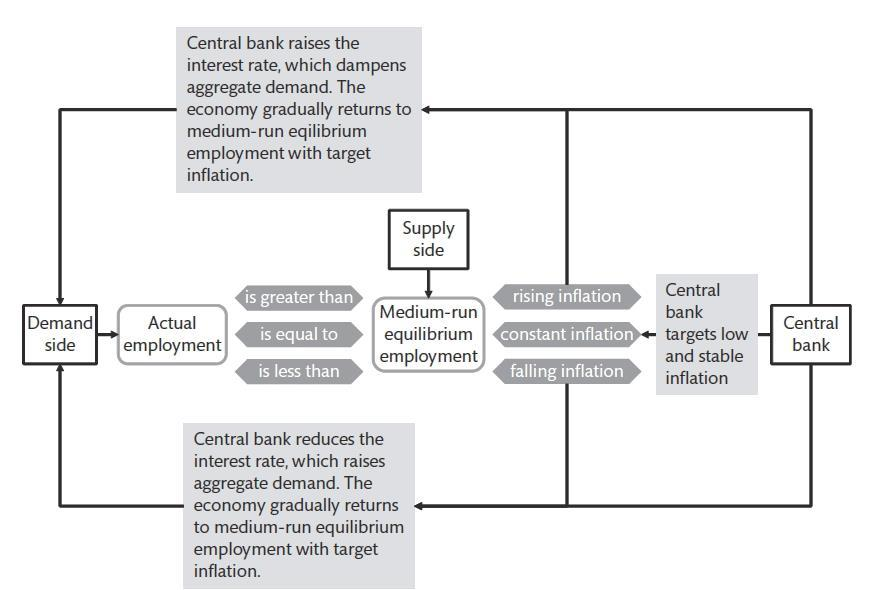
\includegraphics[width=.65\textwidth]{./figures/aula15_fig3.jpg}}
        \caption{Visão esquemática do modelo macro. Fonte: \href{https://bookdown.org/robohay/economicsnotes/Figures/Policy/BoEFig.jpg}{Carlin e Soskice (2015)}}
    \end{figure}
\end{frame}

\begin{frame}
    {Introdução}
    \begin{itemize}
        \item A figura mostra DA e OA e evidencia o papel que um BC operando em um regime de metas de inflação pode ter na resposta a um choque que desvia a economia do equilíbrio de médio prazo\bigskip
        \item O BC aumenta a taxa de juros em resposta a uma taxa de inflação que estiver acima da meta, para amortecer a demanda agregada\bigskip
        \item E reduz a taxa de juros quando a inflação estiver abaixo da meta
    \end{itemize}
\end{frame}

\begin{frame}
    {Introdução}
    \begin{quote}
        Leva tempo até que a política monetária tenha impacto completo sobre a inflação e a economia real. A política monetária é, portanto, guiada por previsões dos desenvolvimentos econômicos.
    \end{quote}
    \begin{flushright}
        \href{https://archive.riksbank.se/Upload/Dokument_riksbank/Kat_publicerat/Rapporter/2010/Monetary_policy_2010.pdf}{Monetary policy in Sweden, Sveriges Riksbank (2010)}
    \end{flushright}
    \begin{itemize}
        \item Uma característica crucial dos regimes modernos de política monetária é que o BC é \hlight{\emph{forward-looking}}\bigskip
        \item O BC faz \textcolor{purple}{previsões} de inflação ao analisar o que está acontecendo em uma economia e deve, ainda, levar em consideração as defasagens envolvidas entre mudanças no instrumento de política monetária (taxa nominal de juro) e o impacto que estas variações terá sobre a atividade econômica
    \end{itemize}
\end{frame}

\begin{frame}
    {Introdução}
    \begin{enumerate}
        \item Qual objetivo o BC deseja alcançar?\medskip
        \item Como o BC pensa a respeito das restrições impostas pelo comportamento do setor privado com que se depara?\medskip
        \item Como o BC implementa sua política?\medskip
    \end{enumerate}
    \begin{itemize}
        \item Quando estas informações são conhecidas, podemos construir um modelo esquemático de comportamento do BC, possibilitando a análise de como responderá a uma variedade de choques\bigskip
        \item Estas respostas podem ser resumidas sob a forma de uma \textcolor{purple}{regra simples de política monetária}\bigskip
        \item Modelo de 3 equações:
        \begin{enumerate}
            \item Regra de política monetária (MR)\medskip
            \item Demanda agregada (IS)\medskip
            \item Oferta sob a forma de uma curva de Phillips (PC)
        \end{enumerate}
    \end{itemize}
\end{frame}

\begin{frame}
    {Introdução}
    \hlight{Qual objetivo o BC deseja alcançar?}\medskip
    \begin{itemize}
        \item Assume-se que o objetivo é usar a política monetária para estabilizar a economia (mantê-la próxima do produto agregado de equilíbrio de médio prazo e a inflação próxima à meta)\bigskip
        \item BC pode ser penalizado caso não atinja seu objetivo de manter inflação na meta\bigskip
        \item UK: se inflação desvia mais do que 1 p.p. (para cima ou para baixo) da meta de 2\%, o presidente do BoE deve escrever uma carta aberta ao chanceler do Tesouro explicando os motivos por não ter cumprido o objetivo e apresentar um plano para retornar a inflação à meta\bigskip
        \item Isso é custoso em termos de reputação para o BoE\bigskip
        \item Quanto mais próximo estiver a economia do PIB de equilíbrio e a inflação da meta, menor os custos em termos de reputação
    \end{itemize}
\end{frame}

\begin{frame}
    {Introdução}
    \textcolor{blue}{Metas de inflação no Brasil}\medskip
    \begin{itemize}
        \item A meta para a inflação é anunciada publicamente e funciona como uma âncora para as expectativas dos agentes sobre a inflação futura, permitindo que desvios da inflação em relação à meta sejam corrigidos ao longo do tempo assegurando, assim, uma inflação baixa e estável\bigskip
        \item A meta se refere à inflação acumulada no ano e é definida pelo CMN. Cabe ao BC agir para alcançá-la\bigskip
        \item O CMN define, em junho, a meta para a inflação com três anos de antecedência. Esse prazo de antecedência reduz as incertezas em relação à inflação futura
    \end{itemize}
\end{frame}

\begin{frame}
    {Introdução}
    \textcolor{blue}{Metas de inflação no Brasil}\medskip
    \begin{itemize}
        \item Se a inflação ao final do ano se situar fora do intervalo de tolerância, o presidente do BC tem de divulgar publicamente as razões do descumprimento, por meio de carta aberta ao ministro da Economia, presidente do CMN, contendo descrição detalhada das causas do descumprimento, as providências para assegurar o retorno da inflação aos limites estabelecidos e o prazo no qual se espera que as providências produzam efeito
    \end{itemize}
\end{frame}

\begin{frame}
    \begin{figure}
        \href{https://www.bcb.gov.br/content/acessoinformacao/SiteAssets/Lists/PerguntasFrequentes/NewForm/Imagem4.png}{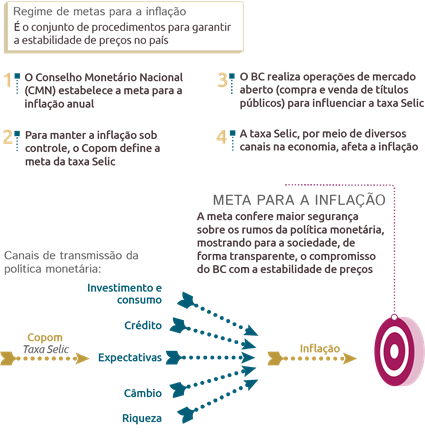
\includegraphics[width=.45\textwidth]{./figures/aula16_fig1.png}}
        \caption{Regime de metas de inflação no Brasil. Fonte: \href{https://www.bcb.gov.br/content/acessoinformacao/SiteAssets/Lists/PerguntasFrequentes/NewForm/Imagem4.png}{Banco Central do Brasil}}
    \end{figure}
\end{frame}

\begin{frame}
    {Introdução}
    \hlight{O que pode impedir que o BC atinja sua meta?}\medskip
    \begin{itemize}
        \item A economia é afetada por choques de demanda e de oferta que, por sua vez, impactam produto agregado e inflação\bigskip
        \item Um choque positivo não antecipado, e.g., que pressiona o produto acima do de equilíbrio de médio prazo, irá aumentar a inflação acima da meta, à medida que fortalece a posição dos trabalhadores\bigskip
        \item Este comportamento dos salários é capturado pela curva de Phillips\bigskip
        \item O BC, então, deve levar este comportamento em consideração, incluindo a persistência da inflação, quando estiver formulando sua resposta ao choque inicial
    \end{itemize}
\end{frame}

\begin{frame}
    {Introdução}
    \hlight{Como o BC traduz seus objetivos em política monetária?}\medskip
    \begin{itemize}
        \item Usa uma regra de política monetária\bigskip
        \item Esta regra pode ser representada no mesmo diagrama da curva de Phillips\bigskip
        \item Mostrará como o BC escolherá sua resposta política preferida dadas as restrições com que se depara a partir dos comportamentos de fixadores de preços e de salários (capturados por uma curva de Phillips em particular)
    \end{itemize}
\end{frame}

\begin{frame}
    {Introdução}
    \begin{itemize}
        \item Na prática, para implementar sua resposta política, o BC realiza um diagnóstico do choque e seus efeitos estimados sobre inflação e produto\bigskip
        \item Usará esta informação, junto às suas preferências por estabilização, para estimar o hiato do produto que está desejando alcançar\bigskip
        \item A curva MR ilustra a melhor resposta do BC ao choque realizado\bigskip
        \item O BC, então, usa a relação entre taxa de juros e produto agregado (na curva IS) para implementar suas escolhas
    \end{itemize}
\end{frame}

\section{Aplicação: \emph{boom} de consumo}
\begin{frame}
    \begin{figure}
        \href{https://bookdown.org/robohay/economicsnotes/Figures/Policy/demandshock.jpg}{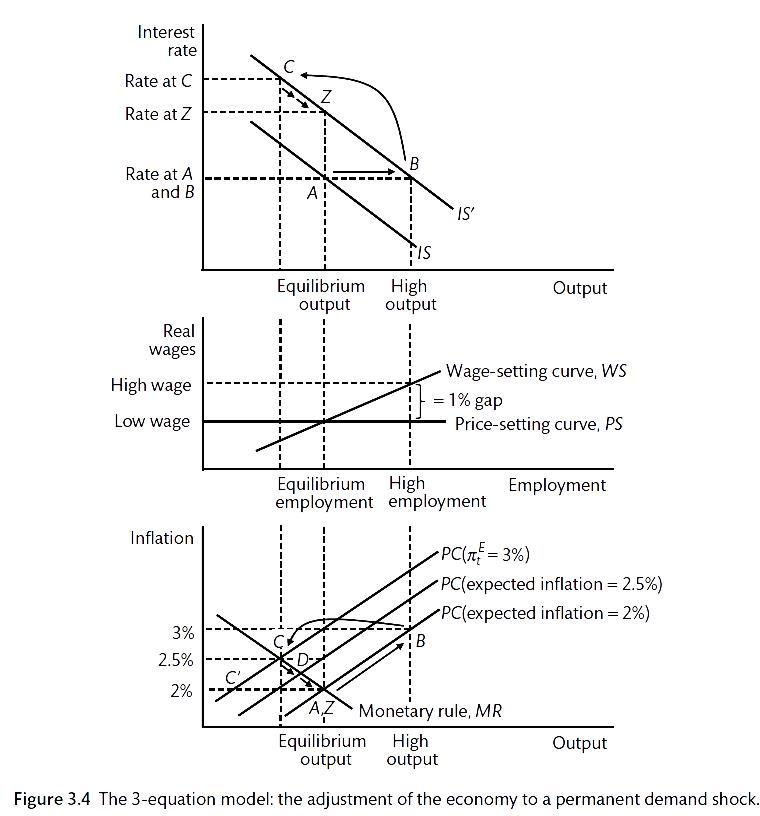
\includegraphics[width=.45\textwidth]{./figures/aula16_fig2.jpg}}
        \caption{Modelo de 3 equações: ajuste a um choque de demanda permanente. Fonte: \href{https://bookdown.org/robohay/economicsnotes/Figures/Policy/demandshock.jpg}{Carlin e Soskice (2015)}}
    \end{figure}
\end{frame}

\begin{frame}
    {Modelo de 3 equações: \emph{boom} de consumo}
    \begin{enumerate}
        \item Choque exógeno de DA: deslocamento da IS\medskip
        \item Maior demanda traduz-se em maiores produto e emprego\medskip
        \item Salários aumentam em 3\%: aumento de 2\% como compensação pela inflação e aumento de 1\% refletindo fortalecimento dos trabalhadores no mercado de trabalho\medskip
        \item Para assegurar margens de lucro, firmas aumentam preços em 3\%\medskip
        \item Deslocamento da curva de Phillips quando expectativas inflacionárias variam (trabalhadores osbservam inflação de 3\% e esperam que permaneçam em 3\% no futuro)
    \end{enumerate}
\end{frame}

\begin{frame}
    {Modelo de 3 equações: \emph{boom} de consumo}
    \begin{enumerate}
        \item[6] BC determinará o quão rápido trazer inflação de volta para a meta, isto determinará o formato da curva de \hlight{regra de política monetária (MR)}. O BC usará o modelo novo-Keynesiano para determinar a taxa de juros que irá trazer a inflação de volta para a meta\medskip
        \item[7] A taxa de juros irá aumentar o suficiente para amortecer a atividade econômica até o ponto em que expectativas inflacionárias sejam reduzidas ao nível inicial\medskip
        \item[8] À medida que expectativas inflacionárias vão se reduzindo, salários e preços aumentam a uma taxa mais baixa\medskip
        \item[9] Enquanto isso acontece, BC reajusta a taxa de juros e guia a economia de volta ao nível de equilíbrio\medskip
        \item[10] No entanto, no novo equilíbrio a taxa de juros será mais elevada. Requer-se um nível mais baixo de investimento para compensar o \emph{boom} de consumo permanente
    \end{enumerate}
\end{frame}

\section{Metas de inflação e política monetária}
\begin{frame}
    {Regimes de metas de inflação e política monetária moderna}
    \begin{itemize}
        \item \href{https://www.rba.gov.au/publications/bulletin/1999/may/pdf/bu-0599-2.pdf}{Glenn Stevens (Reserve Bank of Australia, 1999)} sobre o que aprendemos de política monetária:\medskip
        \begin{enumerate}
            \item Política monetária afeta primordialmente, se não somente, preços (e não atividade econômica) no médio prazo\medskip
            \item Afeta atividade econômica no curto prazo\medskip
            \item Dadas as defasagens, política monetária tem de ser \emph{forward-looking}\medskip
            \item Futuro é incerto, assim como os impactos de mudanças na condução de política sobre a economia\medskip
            \item Expectativas importam: transparência e comunicação do BC são fundamentais\medskip
            \item Um grau adequado de independência operacional para o BC na condução de política monetária é importante
        \end{enumerate}
    \end{itemize}
\end{frame}

\section{Regra de política monetária}
\begin{frame}
    {Introdução}
    \begin{itemize}
        \item Metodologia para derivar regra de política monetária:\medskip
        \begin{enumerate}
            \item \hlight{Preferências do BC} em termos de \textcolor{purple}{função utilidade (ou função perda)} que captura custos incorridos de desvios da meta e do produto de equilíbrio. Isto produz as curvas de indiferença do BC no espaço produto $\times$ inflação e mostra o que o BC gostaria de fazer para estar próximo à meta e do PIB potencial\medskip
            \item \hlight{Restrições} com as quais o BC se depara a partir do lado de oferta: curva de Phillips. Evidencia o \emph{trade-off} objetivo entre inflação e desemprego no curto prazo e determina o que é factível para o BC atingir\medskip
            \item \hlight{Melhor resposta de regra de política monetária} no espaço produto $\times$ inflação: curva MR. Para dada curva de Phillips com que o BC se depara, a regra de política monetária mostra a combinação produto-inflação desejada\medskip
            \item Determinada a posição desejada pelo BC na curva MR, usa-se a curva IS para implementar esta escolha, dado que a IS mostra a taxa de juros que está associada ao nível de PIB escolhido. A taxa de juros é o instrumento de política monetária para influenciar a DA
        \end{enumerate}
    \end{itemize}
\end{frame}

\begin{frame}{Preferências do Banco Central}
    \begin{tabular}{cl}
        \begin{tabular}{c}
            \href{https://en.wikipedia.org/wiki/John_B._Taylor}{
\includegraphics[width=3.5cm]{./figures/aula16_fig3.jpg}}            
        \end{tabular}
         & \begin{tabular}{l}
               \parbox{0.6\linewidth}{%  change the parbox width as appropiate
                   \begin{itemize}
                    \item Como determinar as preferências do BC?\bigskip
                    \item Podemos inferir as preferências do BC a partir de seu comportamento\bigskip
                    \item Via análise empírica do comportamento do Federal Reserve, John Taylor inferiu uma regra de política monetária\bigskip
                    \item A \hlight{regra de Taylor} pode ser derivada a partir de um modelo no qual o BC minimiza flutuações ao redor da meta de inflação e o tamanho do hiato do produto\bigskip
                    \item Utilizaremos esta função perda para elucidar a forma com que BCs se comportam
                    \end{itemize}
               }
           \end{tabular} \\
    \end{tabular}
\end{frame}

\begin{frame}
    {Preferências do Banco Central}
    \begin{itemize}
        \item Função perda do BC para derivar curvas de indiferença (representação do trade-off entre inflação estar distante da meta e produto distante do de equilíbrio)\bigskip
        \item Assume-se, inicialmente, que o BC deseja minimizar flutuações ao redor da meta de inflação $\pi^T$:
        \begin{equation*}
            (\pi_t - \pi^T)^2
        \end{equation*}        
        \begin{enumerate}
            \item BC preocupa-se em evitar tanto inflação abaixo da meta quanto acima da meta\medskip
            \item O peso que o BC dá para trazer a inflação de volta para a meta é maior quanto mais distante a inflação estiver da meta
        \end{enumerate}
    \end{itemize}
\end{frame}

\begin{frame}
    {Preferências do Banco Central}
    \begin{itemize}
        \item BC também preocupa-se em manter PIB próximo ao nível de equilíbrio de médio prazo\medskip
        \item Assume-se que o BC busca minimizar o hiato entre $y_t$ e $y_e$ de forma a auxiliar no objetivo de convergir para a meta de inflação
        \begin{equation*}
            \left(y_t - y_e\right)^2
        \end{equation*}
        \item Observa-se atitude simétrica com relação aos desvios do nível de PIB de equilíbrio\bigskip
        \begin{enumerate}
            \item BC compreende modelo e percebe que inflação só é constante quando $y_t = y_e$\medskip
            \item Se $y_t < y_e$, então, isso representa desemprego desnecessário que deve ser eliminado\medskip
            \item Se $y_t > y_e$, então, esta situação é insustentável e requer aumentos custosos no desemprego para trazer inflação de volta à meta
        \end{enumerate}
    \end{itemize}
\end{frame}

\begin{frame}
    {Preferências do Banco Central}
    \begin{itemize}
        \item A \hlight{função perda do Banco Central} é, portanto:
        \begin{equation*}
            L = \left(y_t - y_e\right)^2 + \beta \left(\pi_t - \pi^T\right)^2,
        \end{equation*}
        onde $\beta$ é o peso relativo atribuído à perda devida à inflação\bigskip
        \item O parâmetro $\beta$ é um parâmetro crítico ao modelo\bigskip
        \item Se $\beta > 1$, o BC atribui um peso relativo menor a desvios no emprego com relação ao seu nível de equilíbrio do que em desvios na inflação, e vice-versa\bigskip
        \item Um BC mais averso com relação à inflação é caracterizado por um $\beta$ mais elevado\bigskip
        \NB{\emoji{warning} As prefer\^{e}ncias do BC podem ser representadas desta maneira simples se assumirmos que a taxa de desconto do BC \'{e} infinita. Isto significa que ele considera apenas um per\'{i}odo de cada vez quando est\'{a} tomando suas decis\~{o}es}
    \end{itemize}
\end{frame}

\begin{frame}
    \begin{figure}
        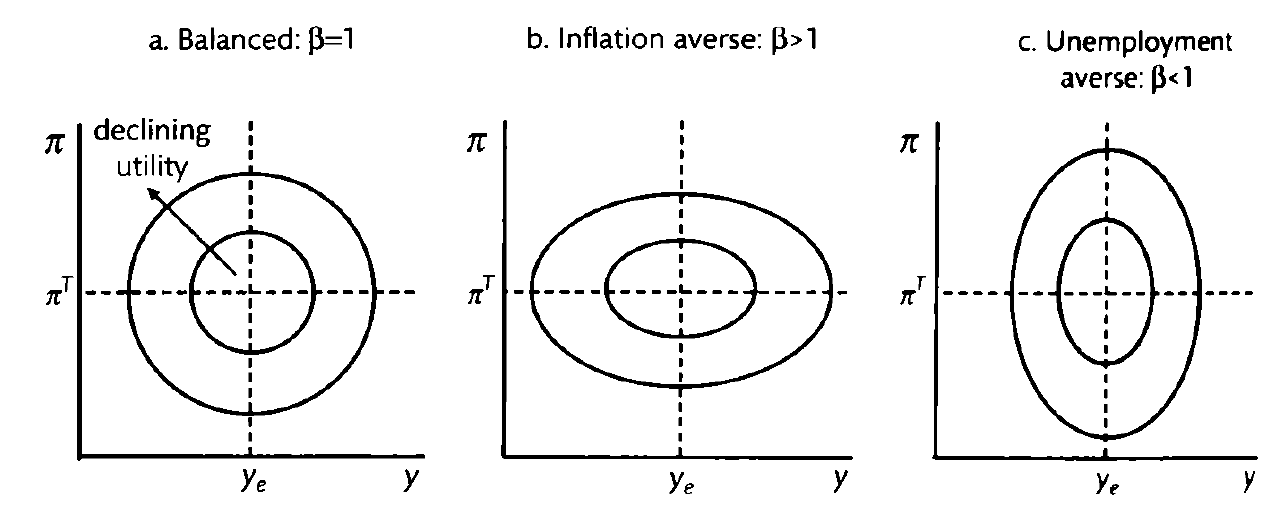
\includegraphics[width=\textwidth]{./figures/aula16_fig4.PNG}
        \caption{Funções perda do Banco Central. Fonte: Carlin e Soskice (2015)}
    \end{figure}
\end{frame}

\begin{frame}
    {Preferências do Banco Central}
    \begin{itemize}
        \item Se $\beta = 1$, o BC é igualmente preocupado com desvios da inflação e do produto com relação às suas metas\bigskip
        \item Neste caso, as curvas de indiferença são círculos de centro $(y_e, \pi^T)$\bigskip
        \item A perda do BC declina à medida que os círculos diminuem\bigskip
        \item Quando $\pi_t = \pi^T$ e $y_t = y_e$, o círculo contrai em um único ponto (\hlight{bliss point}) e a perda é mínima (zero)\bigskip
        \item Neste caso, o BC é indiferente entre uma inflação 1\% acima (ou abaixo) de $\pi^T$ e PIB 1\% abaixo (ou acima) de $y_e$
    \end{itemize}
\end{frame}

\begin{frame}
    {Preferências do Banco Central}
    \begin{itemize}
        \item Se $\beta > 1$, o BC é \hlight{averso à inflação}\bigskip
        \item Isto torna as curvas de indiferença elipsoides\bigskip
        \item Curvas são achatadas para refletir o \emph{trade-off} que o BC está disposto a aceitar entre uma pequena queda na inflação com um aumento elevado no desemprego acima do de equilíbrio\bigskip
        \item Um BC com menos aversão à inflação ($\beta < 1$) terá curvas de indiferença em forma de elipsoides mas com uma orientação vertical, ao invés de horizontal\bigskip
        \item Neste caso, as curvas de indiferença são mais íngremes, refletindo o fato de que o BC só está disposto a trocar uma queda na inflação por uma queda mais baixa no desemprego que nos outros dois casos
    \end{itemize}
\end{frame}

\begin{frame}
    {Preferências do Banco Central}
    \begin{itemize}
        \item Se o BC preocupa-se apenas com a inflação, então, as elipses de perda tornam-se unidimensionais ao longo da linha em $\pi_t = \pi^T$\bigskip
        \item O valor de $\beta$ não reflete se o BC foca em atingir uma meta de inflação ou uma meta de produto\bigskip
        \item Ao invés disso, um BC com um $\beta$ mais baixo está disposto a aceitar um \emph{trade-off} de um período mais longo durante o qual a inflação está distante da meta para reduzir o impacto sobre o desemprego da trajetória de ajuste de retorno ao equilíbrio que teria um BC com maior aversão à inflação
    \end{itemize}
\end{frame}

\begin{frame}
    {A restrição da curva de Phillips}
    \begin{itemize}
        \item A curva de Phillips é uma restrição para o BC pois mostra as combinações de produto e inflação que o BC pode escolher para um dado nível de inflação esperada\bigskip
        \item Dito de outra forma, em qualquer período o BC pode escolher a localização da economia apenas em um ponto sobre a PC com a qual se depara\bigskip
        \item Assumiremos, aqui, uma curva de Phillips sob hipótese de expectativas adaptativas:
        \begin{eqnarray}
            \pi_t &=& \pi_t^E + \alpha(y_t - y_e) \nonumber \\
            &=& \pi_{t-1} + \alpha(y_t - y_e)
        \end{eqnarray}
        \emoji{warning} Outros métodos de formação de expectativas com relação à inflação serão estudadas na disciplina de Macroeconomia III
    \end{itemize}
\end{frame}

\begin{frame}
    \begin{figure}
        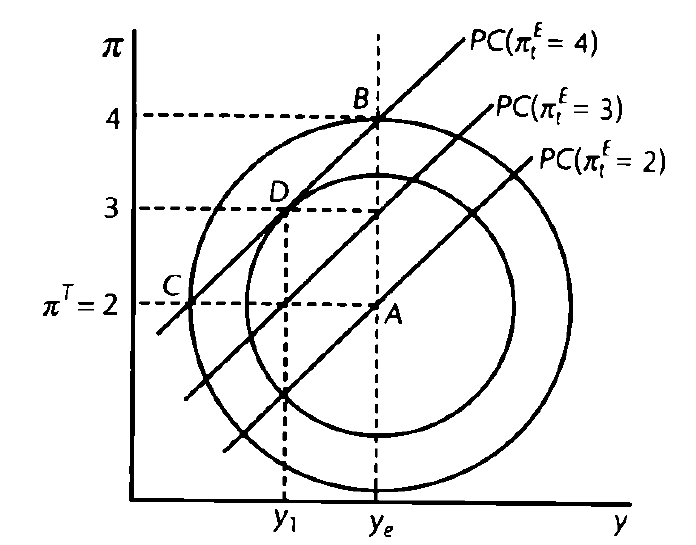
\includegraphics[width=.6\textwidth]{./figures/aula16_fig5.PNG}
        \caption{Círculos de perda e curvas de Phillips. Fonte: Carlin e Soskice (2015)}
    \end{figure}
\end{frame}

\begin{frame}
    {A restrição da curva de Phillips}
    \begin{itemize}
        \item A figura anterior mostra as curvas de Phillips que impõem a restrição do setor privado ao BC\bigskip
        \item Assumimos que $\alpha = 1$, de forma que cada curva de Phillips tem inclinação de 45º\bigskip
        \item Assumindo que $\pi^E = \pi_{t-1} = \pi^T = 2\%$, o BC pode escolher o \hlight{bliss point} $A (\pi^T, y_e)$ no qual a perda é zero\bigskip
        \item Se o sistema econômico é afetado por um choque inflacionário que desvia a inflação da meta, o que acontece? \bigskip
        \item Supondo que a inflação defasada seja de 4\%, ou seja, $PC(\pi_t^E = 4\%)$, temos algumas situações:\medskip
        \begin{enumerate}
            \item Política monetária plenamente acomodativa: único objetivo é atingir a meta de produto $\beta = 0$ (ponto B)\medskip
            \item Política monetária plenamente não acomodativa: único objetivo é atingir a meta de inflação (ponto C)\medskip
            \item Pela figura, é evidente que dadas as preferências do BC, o ponto que minimiza a função perde é o ponto D (tangência entre curvas de indiferença e PC)
        \end{enumerate}
    \end{itemize}
\end{frame}

\begin{frame}
    {Curva de regra de política monetária: abordagem gráfica}
    \begin{itemize}
        \item A \hlight{curva de regra de política monetária (MR)} mostra a combinação produto-inflação preferida pelo BC para qualquer curva de Phillips com que se depara\bigskip
        \item Pode ser derivada graficamente através dos pontos de tangência entre as curvas de Phillips e os círculos de perda\bigskip
        \item A interpolação dos pontos de tangência, que minimizam a função perda do BC dadas as curvas de Phillips, nos dá a curva MR
    \end{itemize}
\end{frame}

\begin{frame}
    \begin{figure}
        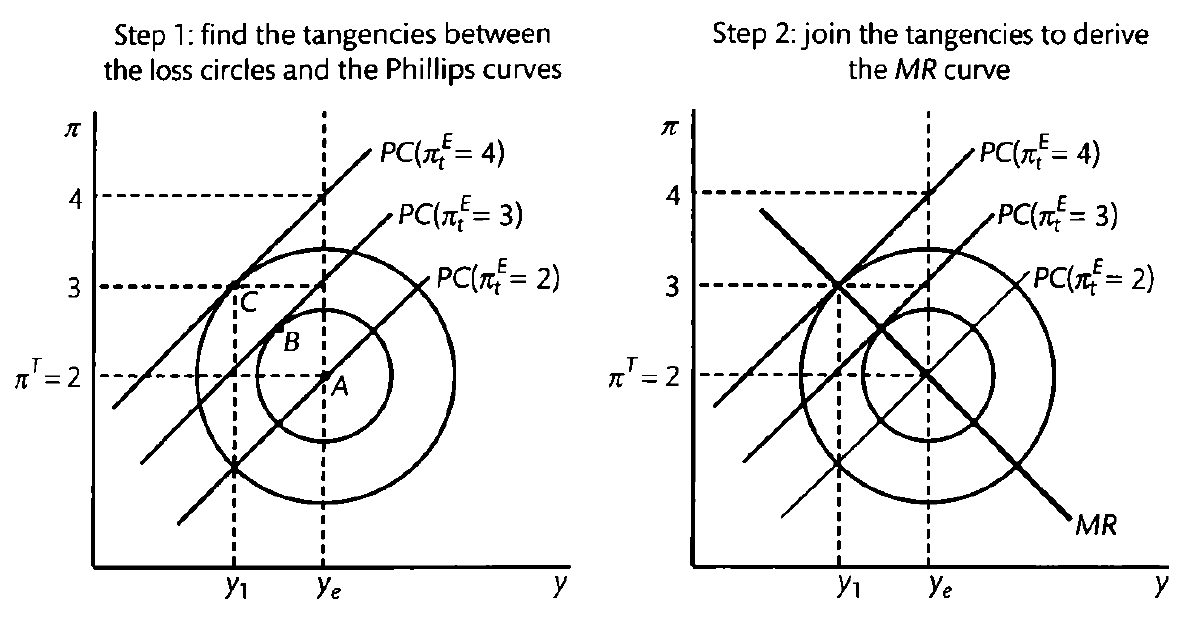
\includegraphics[width=.9\textwidth]{./figures/aula16_fig6.PNG}
        \caption{Derivação gráfica da curva MR. Fonte: Carlin e Soskice (2015)}
    \end{figure}
\end{frame}

\begin{frame}
    {Curva de regra de política monetária: abordagem formal}
    \begin{itemize}
        \item A regra de política monetária pode ser derivada formalmente usando as equações de função perda e curva de Phillips (\hlight{derivação na lousa})\bigskip
        \item A equação da curva MR é dada por:
        \begin{equation}
            (y_t - y_e) = -\alpha\beta(\pi_t - \pi^T)
        \end{equation}
        \item Esta regra de política monetária diz qual hiato do produto o BC deveria escolher quando observa um desvio da inflação com relação à sua meta\bigskip
        \item \textcolor{purple}{Regras de política monetária} usadas pelos BCs são, frequentemente, descritas como \textcolor{blue}{regras de Taylor}\bigskip
        \item A diferença é que a regra de Taylor é expressa em termos da taxa de juros que o BC deveria fixar para implementar o hiato do produto desejado
    \end{itemize}
\end{frame}

\begin{frame}
    {Modelo de 3 equações}
    \begin{itemize}
        \item Para encontrar a taxa de juros que o BC deveria escolher uma vez que decidiu o hiato do produto preferido usando a curva MR, precisamos introduzir a curva IS\bigskip
        \item Com isso, completa-se o modelo de três equações:\bigskip
        \begin{enumerate}
            \item Curva de Phillips (PC)\medskip
            \item Regra de política monetária (MR)\medskip
            \item Demanda agregada (IS)
        \end{enumerate}
    \end{itemize}
\end{frame}

\begin{frame}
    {Implementação da política monetária: curva IS}
    \begin{itemize}
        \item Analisamos o processo pelo qual o BC determina o hiato do produto preferível em resposta a um choque exógeno ao sistema econômico\bigskip
        \item O instrumento que o BC utiliza para implementar a política monetária é a taxa de juros real, $r$\bigskip
        \item O fato de que o BC deve ajustar a \textcolor{purple}{taxa de juros nominal} que possibilitará a determinação de uma \textcolor{blue}{taxa de juros real} particular na curva IS é chamado de \hlight{princípio de Taylor}
    \end{itemize}
\end{frame}

\begin{frame}
    {Implementação da política monetária: curva IS}
    \begin{itemize}
        \item A taxa de juros real é escolhida de forma a assegurar o nível apropriado de demanda agregada e, portanto, produto\bigskip
        \item O BC escolhe o melhor ponto ao longo da curva de Phillips com a qual se depara e, de forma a selecionar o nível correto de DA, deve fixar a taxa de juros no nível associado de curva IS\bigskip
        \item A curva IS mostra o efeito de variações na taxa de juros sobre a DA:
        \begin{eqnarray}
            y &=& \kappa(c_0 + a_0 + G) - \kappa a_1 r \nonumber \\
            &=& A - ar,
        \end{eqnarray}
        onde o termo $A$ inclui o multiplicador $\kappa$ e todos os elementos autônomos de DA como gastos do governo e os elementos autônomos e \emph{forward-looking} de consumo e investimento
    \end{itemize}
\end{frame}

\begin{frame}
    {Implementação da política monetária: curva IS}
    \begin{itemize}
        \item No modelo de 3 equações, utilizaremos uma \hlight{curva IS dinâmica} para representar o lado da demanda e capturar o fato de que a DA responde negativamente à taxa de juros real, $r$, com um período de defasagem\bigskip
        \item Exemplo: estimativas do BoE de que o impacto das taxas de juros sobre o produto leva (um máximo de) um ano\bigskip
        \item A curva IS dinâmica é definida da seguinte forma:
        \begin{equation}
            y_t = A - ar_{t-1}
        \end{equation}
    \end{itemize}
\end{frame}

\section{Bibliografia}
\begin{frame}{\emoji{books} Bibliografia}
    \begin{itemize}                        
        \item CARLIN, W.; SOSKICE, D. Macroeconomics: Institutions, instability, and the financial system. Oxford, UK: Oxford University Press, 2015\medskip             
        \item STEVENS, G. \href{https://www.rba.gov.au/speeches/1999/sp-ag-200499.html}{Six years of inflation targeting}. Address to the Economic Society of Australia. Sidney, AUS, 1999\medskip
        \item SVERIGES RIKSBANK. \href{https://archive.riksbank.se/en/Web-archive/Published/Press-Releases/2010/Monetary-Policy-in-Sweden/index.html\#:~:text=Monetary\%20Policy\%20in\%20Sweden\%20Date03\%2F06\%2F2010\%20The\%20document\%20\%22Monetary,from\%20the\%20specification\%20of\%20the\%20monetary\%20policy\%20objective}{Monetary policy in Sweden}, 2010\medskip
        \item TAYLOR, J.B. \href{https://web.stanford.edu/~johntayl/Onlinepaperscombinedbyyear/1993/Discretion_versus_Policy_Rules_in_Practice.pdf}{Discretion versus policy rules in practice}. Carnegie-Rochester Series on Public Policy 39, 1993       
    \end{itemize}
\end{frame}
\end{document}
